\chapter{Diseño del sistema}\label{capitulo5}
En este capítulo se expone el diseño detallado del sistema desarrollado, con el objetivo de proporcionar una visión clara y estructurada de su organización interna. Se abordan los distintos niveles de diseño, desde la arquitectura general del sistema hasta los modelos de datos, pasando por el diagrama entidad-relación (E/R) y la definición de casos de uso.

Cada sección detalla las decisiones técnicas adoptadas durante el proceso de diseño, justificando su adecuación a los requisitos funcionales y no funcionales definidos previamente. 

\section{Diseño de la arquitectura}
La arquitectura general del sistema ha sido diseñada siguiendo una estructura cliente-servidor desacoplada, orientada a servicios, y basada en principios de escalabilidad, mantenibilidad y seguridad. Se compone de tres capas principales:

\begin{enumerate}
    \item \textbf{Frontend (Cliente)}: Desarrollado con ``React.js'', el cliente proporciona una interfaz de usuario interactiva y responsive, diseñada para ser intuitiva y accesible desde dispositivos móviles y de escritorio. La comunicación con el servidor se realiza a través de peticiones HTTP (``API REST'') utilizando JSON como formato de intercambio de datos.

    \item \textbf{Backend (Servidor de aplicaciones)}: Implementado con ``FastAPI'', el servidor expone una API REST que gestiona la lógica de negocio, la validación de datos, la autenticación mediante JWT y la interacción con la base de datos. 

    \item \textbf{Base de datos}: Se utiliza ``MongoDB'', una base de datos NoSQL orientada a documentos, que permite gran flexibilidad para el manejo de datos estructurados y semiestructurados. 
\end{enumerate}

\subsection{Diagrama de arquitectura}
\begin{figure}[H]
    \centering
    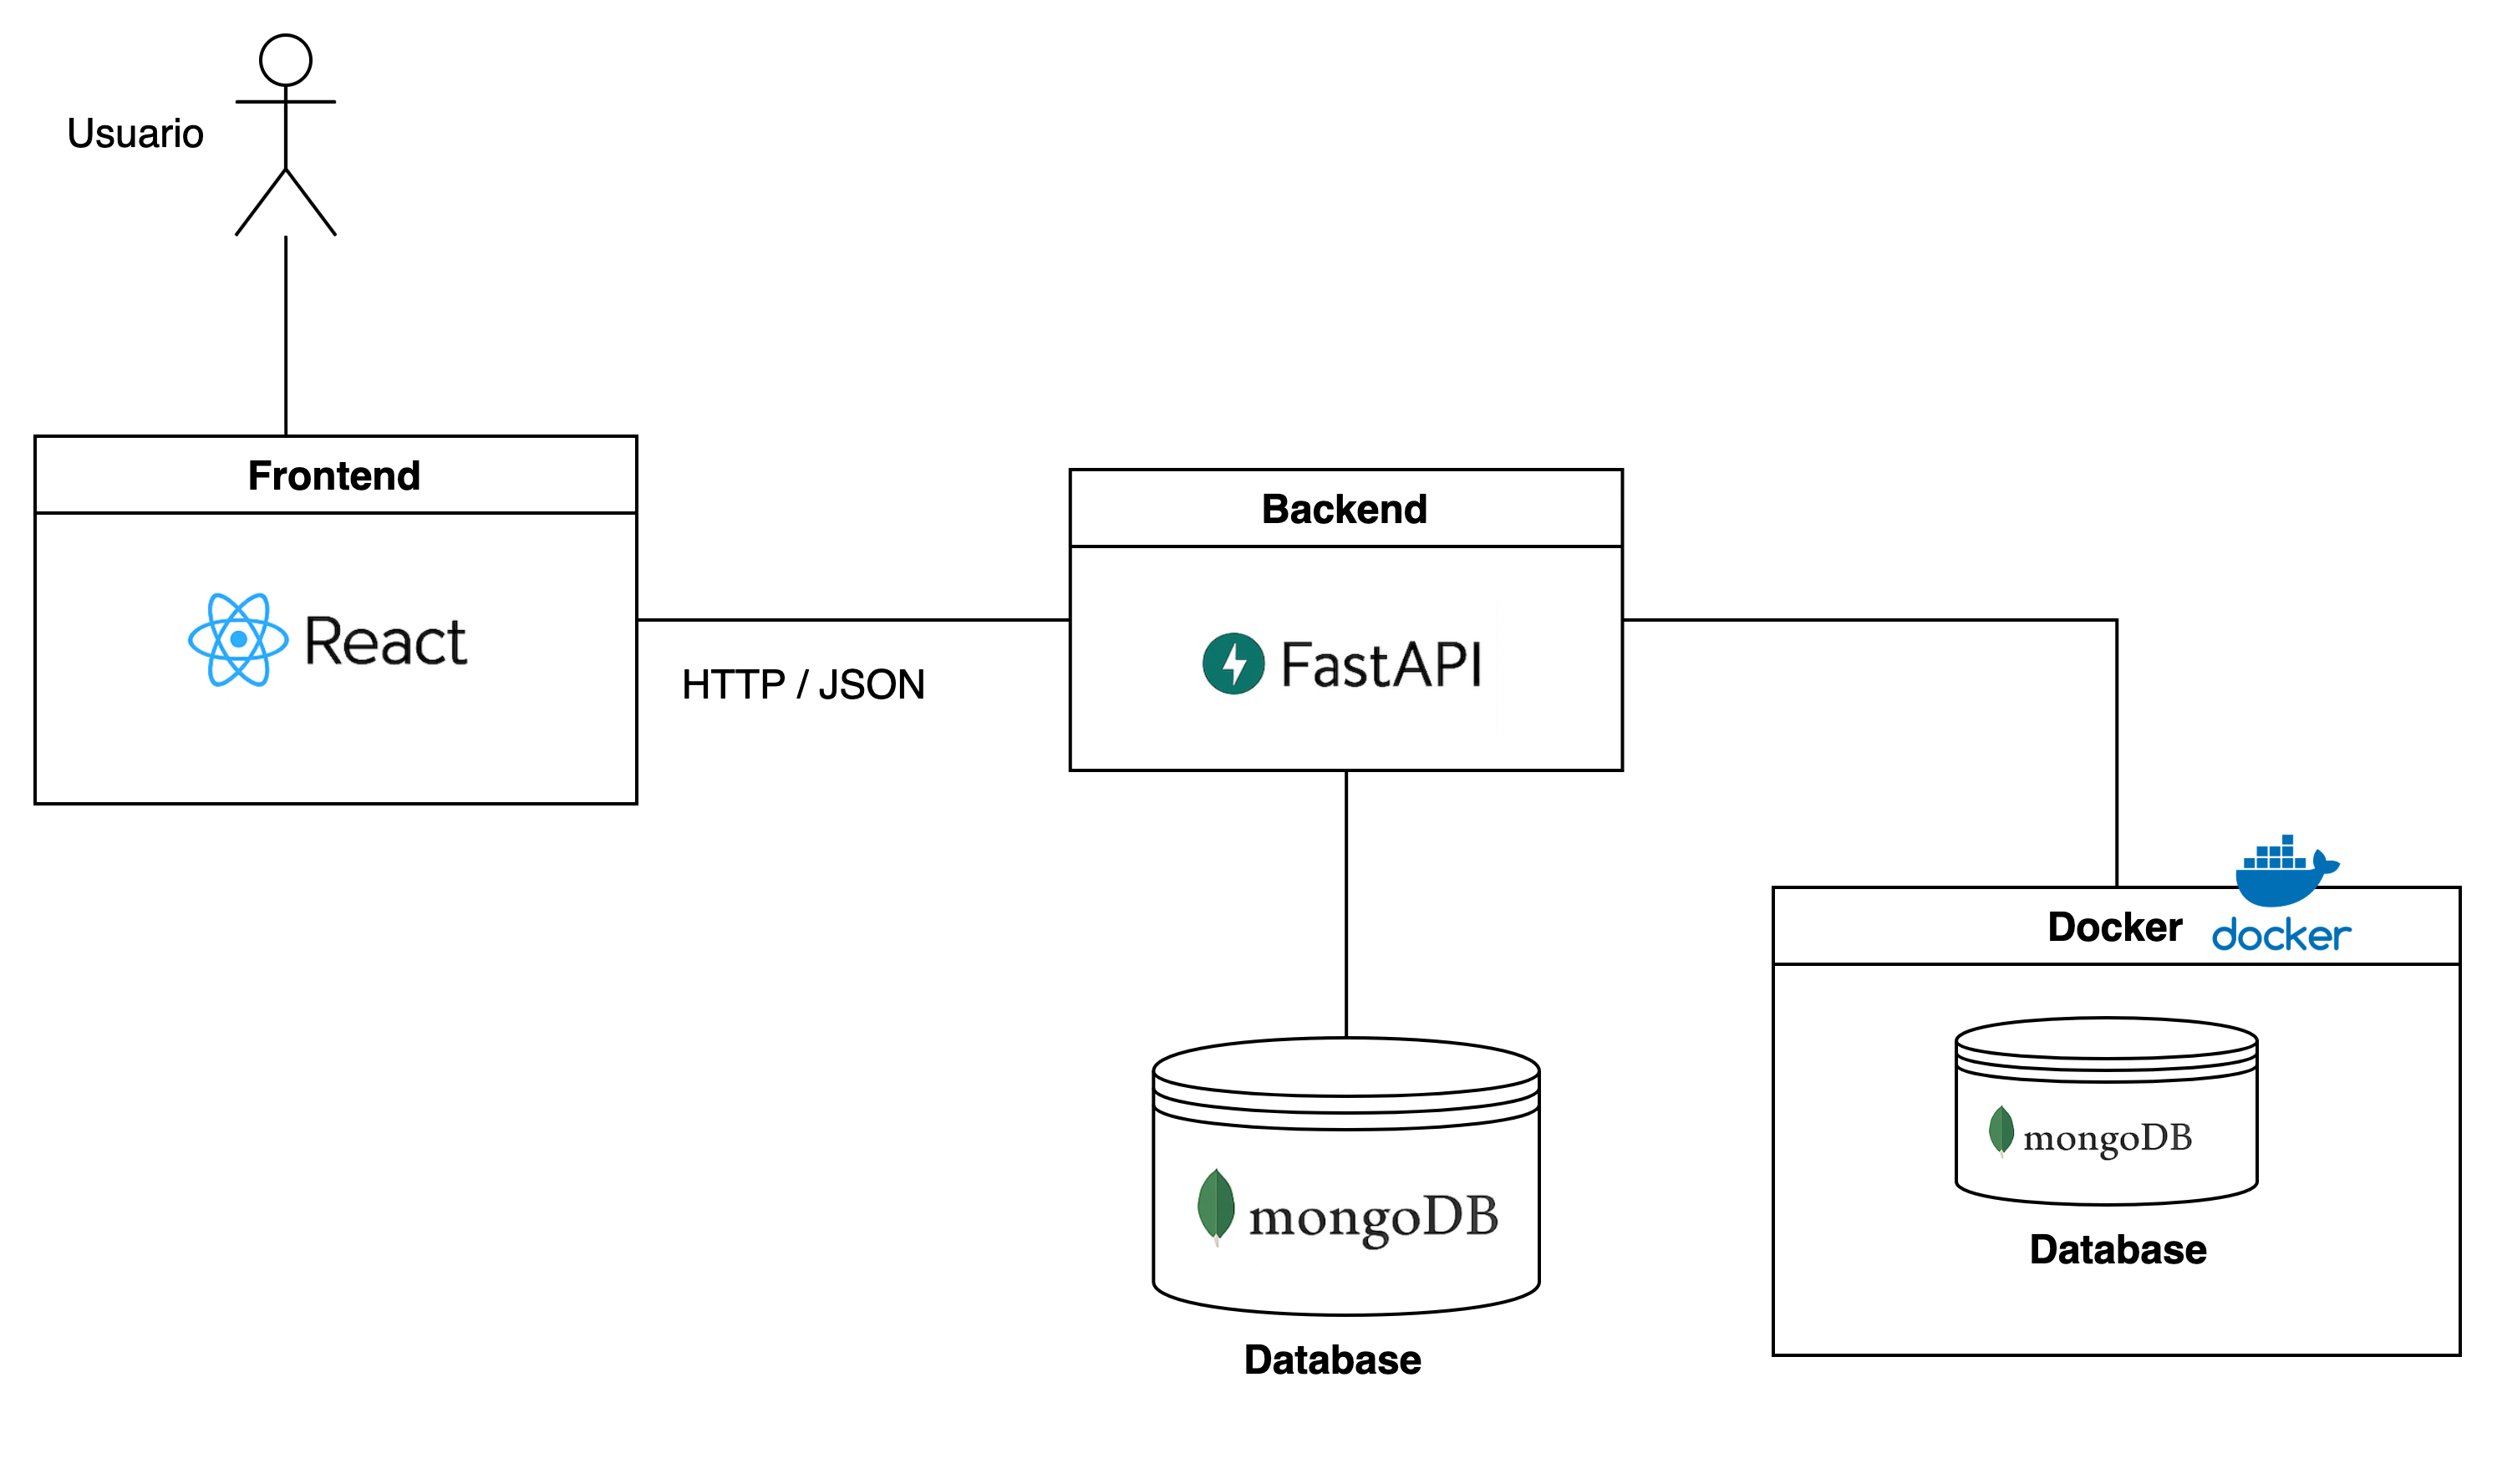
\includegraphics[width=1\linewidth]{Plantilla_TFG_latex/imagenes/D_arquitectura.png}
    \caption{Enter Caption}
    \label{fig:enter-label}
\end{figure}

El usuario interactúa con la interfaz web (React), que a su vez realiza peticiones al backend (FastAPI), el cual consulta y actualiza los datos en la base de datos MongoDB. Todo el flujo está protegido mediante autenticación JWT y se sigue una arquitectura orientada a servicios con separación clara de responsabilidades.

\section{Modelo de Datos}
El modelo de datos define la estructura con la que se organiza, almacena y relaciona toda la información que maneja el sistema. Esta estructura no solo da soporte a las funcionalidades principales de la aplicación, sino que también responde a las necesidades específicas del entorno educativo para el que ha sido desarrollada.

Desde el punto de vista conceptual, el modelo se compone de tres bloques diferenciados, según el origen y propósito de los datos:

\begin{enumerate}
    \item En primer lugar, se integran datos provenientes de fuentes externas, como bases de datos nutricionales reconocidas que proporcionan información precisa sobre la composición de alimentos. 
    
    \item En segundo lugar, se incorpora un conjunto de datos que han sido generados específicamente para el desarrollo de este sistema, entre los que destacan las recetas elaboradas por estudiantes del Grado en Nutrición Humana y Dietética. Estos datos aportan un valor añadido al proyecto, adaptados a las necesidades del entorno educativo.

    \item Por último, se contemplan los datos generados dinámicamente durante la interacción con el sistema, es decir, aquellos que se crean y modifican a medida que los usuarios (nutricionistas o estudiantes) utilizan la aplicación. Aquí se incluyen las entidades como pacientes, dietas, ingestas, usuarios registrados y sus relaciones.
\end{enumerate}

A continuación, se describen las colecciones utilizadas para almacenar los distintos tipos de datos. Entre paréntesis se indica el nombre exacto de cada colección en la base de datos MongoDB. Tanto las entidades como sus atributos se han nombrado en inglés para mantener la coherencia terminológica con fuentes internacionales, facilitar la colaboración global y evitar ambigüedades en un entorno multilingüe.

\subsection{Datos provenientes de fuentes externas}
Los datos que se presentan a continuación provienen de un proyecto previo vinculado al presente trabajo. Han sido recopilados a partir de diversas fuentes externas y sometidos a un minucioso proceso de limpieza y normalización, con el objetivo de asegurar su calidad, consistencia e integridad. Posteriormente, toda la información fue estructurada y almacenada en un contenedor Docker, lo que facilita su acceso, despliegue y gestión a lo largo del desarrollo del sistema.

Dado que este sistema está pensado para ser utilizado por profesionales de la nutrición en el gabinete de la Universidad de Granada, en este proyecto se ha trabajado únicamente con datos de origen español. Esta decisión busca mantener la coherencia cultural y gastronómica, especialmente en lo que respecta a ingredientes, platos típicos y hábitos alimentarios comunes.

Aun así, la estructura del sistema se ha diseñado de forma abierta y adaptable. El modelo de datos es lo bastante general como para permitir la incorporación de nuevas recetas, ya sean propias del entorno local o de otras culturas. De hecho, el sistema ya incluye algunas recetas internacionales, lo que facilita su extensión y adaptación a distintos contextos sin necesidad de cambios estructurales.

Las colecciones formadas a partir de esta fuente de datos son las siguientes(entre paréntesis se indica el nombre exacto de la colección en MongoDB):

\subsubsection*{Ingredientes (``Ingredients'')}
La colección de ingredientes se ha obtenido a partir de una colaboración entre centros de investigación públicos, administraciones e instituciones privadas. Su objetivo común es mantener y desarrollar la Base de Datos Española de Composición de Alimentos (BEDCA).

\begin{table}[t]
    \centering
    \begin{tabular}{|l|p{8cm}|}
        \hline
        \textbf{Campo} & \textbf{Descripción} \\
        \hline
        \texttt{id} & Identificador único del ingrediente (ObjectId o valor asignado) \\
        \hline
        \texttt{name\_Esp} & Nombre del ingrediente en español \\
        \hline
        \texttt{name\_En} & Nombre del ingrediente en inglés \\
        \hline
        \texttt{LanguaL} & Código del sistema de clasificación \textit{LanguaL} asociado al ingrediente \\
        \hline
        \texttt{origin\_ISO} & Código ISO 3166 del país de procedencia del ingrediente \\
        \hline
        \texttt{source} & Fuente o base de datos original de la que procede el ingrediente \\
        \hline
        \texttt{category\_Esp} & Categoría alimentaria del ingrediente (en español) \\
        \hline
        \texttt{category\_En} & Categoría alimentaria del ingrediente (en inglés) \\
        \hline
        \texttt{edible} & Porcentaje comestible del ingrediente respecto a su peso total \\
        \hline
        \texttt{compounds} & Lista de compuestos químicos presentes en el ingrediente (ej. azúcares, grasas, minerales) \\
        \hline
        \texttt{nutritional\_Info\_100gr} & Información nutricional estándar por 100 gramos de ingrediente (kcal, proteínas, carbohidratos, etc.) \\
        \hline
    \end{tabular}
    \caption{Estructura de la colección \texttt{Ingredientes}}
    \label{tab:ingredientes}
\end{table}


\subsubsection{Recetas (``Recipes'')}
La colección de recetas utilizada en este trabajo es una base de datos preexistente, cuya estructura se detalla en la Tabla~\ref{tab:recetas}. Los datos provienen de una fuente denominada Recetas de la Abuela, un corpus desarrollado durante el Hackathon “SomosNLP” celebrado en marzo de 2024, en respuesta a una propuesta centrada en la recopilación de recetas típicas por país o región geográfica. En el presente proyecto nos enfocamos exclusivamente en recetas de origen español. Al tratarse de un conjunto de datos previamente desarrollado, su formato ya está normalizado y estructurado.

\begin{table}
    \centering
    \begin{tabular}{|l|p{8cm}|}
        \hline
        \textbf{Campo} & \textbf{Descripción} \\
        \hline
        \texttt{id} & Identificador único de la receta (ObjectId o UUID) \\
        \hline
        \texttt{language\_ISO} & Código ISO del idioma original de la receta (ej. ``es'', ``en'') \\
        \hline
        \texttt{n\_Diners} & Número de comensales a los que está destinada la receta \\
        \hline
        \texttt{title} & Título o nombre descriptivo de la receta \\
        \hline
        \texttt{URL} & Enlace (URL) a la fuente original o página de referencia de la receta \\
        \hline
        \texttt{category} & Categoría principal asignada a la receta (ej. ``Postre'', ``Plato principal'') \\
        \hline
        \texttt{subcategory} & Subcategoría específica dentro de la categoría (ej. ``Pastas'', \textit{Cremas}) \\
        \hline
        \texttt{minutes} & Tiempo total estimado para la preparación (en minutos) \\
        \hline
        \texttt{n\_Ingredients} & Número total de ingredientes utilizados en la receta \\
        \hline
        \texttt{ingredients} & Lista estructurada de ingredientes utilizados \\
        \hline
        \texttt{n\_Steps} & Número de pasos que componen el procedimiento de elaboración \\
        \hline
        \texttt{steps} & Lista ordenada de instrucciones paso a paso para preparar la receta \\
        \hline
        \texttt{images} & Lista de URLs de imágenes asociadas a la receta \\
        \hline
        \texttt{nutritional\_Info} & Información nutricional estándar por cada 100 gramos de la receta \\
        \hline
        \texttt{tags} & Lista de etiquetas o palabras clave asociadas (ej. ``vegano'', ``sin gluten'') \\
        \hline
        \texttt{aver\_Rate} & Valoración media otorgada por los usuarios \\
        \hline
        \texttt{review\_num} & Número total de valoraciones recibidas \\
        \hline
        \texttt{reviews} & Lista de reseñas o comentarios asociados a la receta \\
        \hline
        \texttt{origin\_ISO} & Código ISO del país o región de origen gastronómico de la receta \\
        \hline
        \texttt{FSA\_Lights\_Per100g} & Semáforo nutricional según la normativa FSA (por 100g) \\
        \hline
        \texttt{WHO\_Lights\_Per100g} & Indicadores nutricionales basados en estándares de la OMS (por 100g) \\
        \hline
        \texttt{dietary\_Preferences} & Lista de criterios dietéticos aplicables (ej. ``vegetariano'', ``diabético'') \\
        \hline
    \end{tabular}
    \caption{Estructura de la colección \texttt{Recetas}}
    \label{tab:recetas}
\end{table}

\subsection*{Ampliación del modelo de recetas}
Durante el desarrollo del sistema, se identificó la necesidad de enriquecer el modelo de datos de las recetas con información más estructurada, coherente y útil para el análisis nutricional automatizado. En la versión inicial, los ingredientes de cada receta estaban vinculados a una base de datos heterogénea, compuesta por entradas procedentes de distintas fuentes normalizadas. 

Con el objetivo de unificar criterios y garantizar una fuente confiable, se tomó la decisión de adoptar exclusivamente la base de datos BEDCA (Base de Datos Española de Composición de Alimentos) como referencia oficial para todos los ingredientes del sistema.
Esta decisión implicó una transformación progresiva del campo ``ingredients'', orientada a vincular cada entrada con un identificador único de la colección BEDCA, y a estandarizar la información contenida.

Para llevar a cabo este proceso de vinculación, se desarrolló un sistema de emparejamiento semántico utilizando modelos de lenguaje entrenados en español. Este sistema permitió analizar los textos originales de los ingredientes y compararlos con los registros de BEDCA, determinando cuál era el más similar en cada caso. El emparejamiento se hizo considerando tanto el nombre principal del ingrediente como los detalles adicionales (por ejemplo, tipo de corte, cocción o presentación), con el objetivo de obtener coincidencias lo más precisas posible.

Una vez establecido el vínculo con BEDCA, se incorporó un nuevo campo a las recetas: ``nutritional\_info'', que contiene el perfil nutricional total de la receta, calculado automáticamente a partir de los ingredientes estandarizados. Este cálculo tiene en cuenta la proporción estimada de cada ingrediente en gramos, lo que permite reflejar con precisión su contribución real al valor energético, contenido en proteínas, hidratos de carbono, grasas, vitaminas y minerales.

Este nuevo campo se almacena directamente en la base de datos de recetas para evitar tener que recalcular los datos nutricionales en cada consulta. Esta decisión está motivada por cuestiones de eficiencia: calcular esta información en tiempo real sería demasiado costoso en términos de rendimiento, especialmente si se consulta con frecuencia o en contextos educativos donde múltiples usuarios acceden simultáneamente.

\section{Datos creados para las funcionalidades del sistema}
Además de integrar datos provenientes de fuentes oficiales, el sistema ha incorporado un conjunto de datos desarrollados de forma específica para dar soporte a las funcionalidades internas y didácticas de la plataforma. Estos datos no existen en fuentes externas, pero son esenciales para el funcionamiento real de la aplicación y para enriquecer la experiencia formativa del alumnado.

Este bloque incluye las recetas originales elaboradas por estudiantes del Grado en Nutrición Humana y Dietética,  las porciones estándar extraídas y normalizadas a partir de documentos docentes e imágenes asociadas a alimentos, obtenidas automáticamente desde plataformas libres de derechos y revisadas manualmente.

\subsection{Recetas diseñadas por estudiantes}

Una de las principales aportaciones originales del sistema es la\textbf{ inclusión de un corpus de recetas generadas por estudiantes del Grado en Nutrición Humana y Dietética.} Estas recetas han sido recogidas, revisadas y normalizadas con el objetivo de integrarlas en la base de datos de forma coherente con la misma estructura de las recetas de fuentes externas. Para cada receta se han documentado atributos como el título, número de comensales, categoría, pasos, ingredientes, etiquetas y valores nutricionales estimados por 100 gramos. La creación de estas recetas se realizó en el contexto de asignaturas prácticas, fomentando así el aprendizaje activo de los estudiantes mediante el diseño y estructuración de menús reales. 

Originalmente, todas las recetas se encuentran recogidas en formato PDF.Para su integración en el sistema, se desarrolló un proceso automatizado de extracción de datos mediante scripts en Python, capaces de identificar las secciones clave de cada receta (como ingredientes, instrucciones o comentarios nutricionales), transformar los textos en estructuras procesables y corregir errores comunes de formato. 

Y después se aplicaron técnicas de procesamiento semántico para vincular automáticamente sus ingredientes con los elementos de la base de datos BEDCA, utilizando modelos de lenguaje como ``sentence-transformers''. 

El uso de estos modelos permite comparar expresiones en lenguaje natural captando similitudes de significado, más allá de coincidencias literales.
Esto resulta especialmente útil cuando los nombres de los ingredientes varían en forma o redacción, pero se refieren a conceptos nutricionalmente equivalentes (por ejemplo, ``azúcar blanco'' y simplemente ``azúcar''). De este modo, se mejora significativamente la precisión en la vinculación automática de ingredientes y se reduce la necesidad de intervención manual.

Este proceso incluyó:
\begin{itemize}
    \item Separación del nombre del ingrediente en componente principal y detalles.
    \item Comparación semántica del ingrediente con los disponibles en BEDCA.
    \item Selección del ingrediente más similar y asignación de su identificador (``ingredientID'') y su nivel de similitud (``max\_similarity'').
\end{itemize}

Una vez vinculado cada ingrediente con su equivalente en la base BEDCA, hay que adaptarla al modelo de datos del sistema para garantizar la coherencia estructural y su correcta integración en la colección de recetas \ref{tab:recetas}. Para ello, se desarrollaron scripts que transformaban estos datos en un formato estandarizado. Dichos scripts reorganizaban la información en campos como calorías, proteínas, hidratos de carbono, grasas, fibra etc., expresados por 100 gramos, y los almacenaban en el campo ``nutritional\_info'' de cada receta.

Esta adaptación permitió integrar de forma uniforme los valores nutricionales ya existentes en el modelo de datos del sistema. Al estructurar esta información según el formato definido, se garantizó su disponibilidad inmediata para todas las funcionalidades, como la visualización en detalle o la generación de menús, sin necesidad de recalcular los datos en cada consulta.

\subsection{Porciones estándar(``food\_portions'')}
Se ha incorporado también una colección dedicada a representar porciones estándar, unidades de consumo habitual y medidas caseras para una amplia variedad de información de alimentos. Esta información permite mejorar la precisión del análisis nutricional, sobre todo en contextos donde los usuarios no disponen del peso exacto del alimento consumido. 

El contenido de esta colección proviene de la tabla proporcionada por el profesorado del Grado en Nutrición Humana y Dietética, extraída de una fuente bibliográfica especializada en dietética clínica. \cite{Aparicio2015raciones}

La tabla fue convertida desde formato PDF a formato estructurado JSON mediante un proceso manual de revisión y limpieza para garantizar la coherencia de los datos. Se eliminaron redundancias, se estandarizaron las categorías y se adaptaron los nombres de alimentos a una forma compatible con el sistema. El resultado se almacenó en una colección denominada ``food\_portions'' ~\ref{tab:foodportions}.

\begin{table}[H]
    \centering
    \begin{tabular}{|l|p{8cm}|}
        \hline
        \textbf{Campo} & \textbf{Descripción} \\
        \hline
        \texttt{category} & Categoría principal del alimento, como “01 Cereales”, “02 Legumbres”, etc. \\
        \hline
        \texttt{subcategory} & Subcategoría específica dentro de la categoría general, por ejemplo, “0101 Granos y harinas”. \\
        \hline
        \texttt{food} & Nombre base del alimento al que se asocian las porciones (por ejemplo, “Arroz”). \\
        \hline
        \texttt{standard\_portion} & Lista de valores en gramos correspondientes a una ración estándar media del alimento. \\
        \hline
        \texttt{units} & Lista de unidades específicas de compra o presentación (por ejemplo, “unidad”, “paquete”) opcional. \\
        \hline
        \texttt{household\_measures} & Lista de medidas caseras habituales como “puñado”, “guarnición”, “sopa”, junto con su peso estimado en gramos. \\
        \hline
    \end{tabular}
    \caption{Estructura de la colección \texttt{food\_portions}}
    \label{tab:foodportions}
\end{table}

Esta colección se utiliza mediante un ``endpoint'' que permite recuperar automáticamente las porciones estándar asociadas a un alimento. Su integración facilita la entrada de datos por parte del usuario, mejora la precisión del cálculo nutricional y ofrece medidas caseras comprensibles, sin renunciar a la coherencia técnica necesaria para el análisis automatizado.

\subsection{Imágenes de ingredientes}

Un problema existente en BEDCA, así como otros conjuntos similares, es la falta de imágenes asociadas. 

Para mejorar la experiencia visual y la usabilidad del sistema, se diseñó un mecanismo automático para asociar imágenes representativas a los alimentos e ingredientes registrados. Esta funcionalidad permite mostrar ilustraciones en los listados y fichas detalladas, facilitando la identificación de productos tanto para estudiantes como para usuarios no especializados.

Con el fin de automatizar y escalar este proceso sin incurrir en problemas de licencias o derechos de autor, se optó por utilizar Pixabay\footnote{Plataforma con licencia gratuita de imagenes. Fuente: \url{https://pixabay.com}.}
, una plataforma de imágenes libres de uso con licencia Creative Commons. La recolección se realiza a través de su API oficial, permitiendo obtener automáticamente imágenes relevantes en función del nombre del alimento en español (``name\_esp'').

\begin{table}[H]
    \centering
    \begin{tabular}{|l|p{8cm}|}
        \hline
        \textbf{Campo} & \textbf{Descripción} \\
        \hline
        \texttt{\_id} & Identificador único del documento (ObjectId). \\
        \hline
        \texttt{name\_esp} & Nombre del ingrediente en español al que está asociada la imagen. \\
        \hline
        \texttt{image\_url} & URL local de la imagen descargada y almacenada en el servidor (\texttt{static/images}). \\
        \hline
    \end{tabular}
    \caption{Estructura de la colección \texttt{ingredient\_image}}
    \label{tab:ingredient_image}
\end{table}

Tras la obtención automática de imágenes mediante la API de Pixabay, se realizó una revisión manual completa de todos los registros almacenados en la colección ``ingredient\_image''. Se detectaron muchos casos en los que las imágenes descargadas no representaban adecuadamente el alimento correspondiente (por ejemplo, imágenes genéricas, irrelevantes o con baja calidad). Dichas imágenes inadecuadas fueron eliminadas de la base de datos y se asignó por defecto el logotipo del sistema, asegurando así una presentación visual homogénea en la interfaz de usuario.

\subsection{Datos generados durante la interacción con el sistema}
Durante el uso de la herramienta se generan diversos datos vinculados a la actividad del usuario, como la creación de ingestas, la planificación de dietas, los cálculos automáticos de requerimientos nutricionales y el registro de pacientes. Estos datos no solo permiten una experiencia personalizada y adaptada a cada caso, sino que también implican la gestión de información sensible de carácter clínico y personal.

Por este motivo, el sistema ha sido diseñado siguiendo principios fundamentales de privacidad y seguridad. La información generada durante la interacción se almacena de forma estructurada en una base de datos protegida, y su acceso está restringido mediante un sistema de autenticación basado en tokens JWT. Solo los usuarios debidamente registrados y autorizados pueden acceder, modificar o eliminar datos relacionados con sus propios pacientes, garantizando así la confidencialidad de la información.

\subsubsection{Nutricionista (``Nutritionist'')}
Esta colección se corresponde al registro de los nutricionistas, es decir, de los profesionales que trabajarán con la aplicación, y sigue la estructura mostrada en la Tabla~\ref{tab:nutritionistas}.

\begin{itemize}
\item El atributo ``password'' almacena la contraseña encriptada para garantizar la seguridad a la hora de autenticación.

\item El atributo ``language'' almacena el idioma de preferencia del usuario para interactuar con el sistema de información nutricional. Actualmente, se puede seleccionar entre español e inglés. Aunque esta preferencia no afecta de forma integral a toda la interfaz del sistema en esta versión, sí tiene una funcionalidad prevista: en futuras implementaciones, el idioma seleccionado influirá en la prioridad de visualización de recetas, mostrando primero aquellas disponibles en el idioma preferido del usuario. No obstante, cabe destacar que esta funcionalidad se encuentra en una fase inicial de diseño y, por el momento, no tiene un uso real activo en el sistema.
\end{itemize}

\begin{table}[t]
    \centering
    \begin{tabular}{|l|p{10cm}|}
        \hline
        \textbf{Campo} & \textbf{Descripción} \\
        \hline
        \texttt{\_id} & Identificador único del nutricionista (``ObjectId'') \\
        \hline
        \texttt{name} & Nombre completo del nutricionista \\
        \hline
        \texttt{email} & Correo electrónico del nutricionista \\
        \hline
        \texttt{password} & Contraseña almacenada de forma encriptada para garantizar la seguridad en el acceso \\
        \hline
        \texttt{phone} & Número de teléfono de contacto del nutricionista \\
        \hline
        \texttt{language} & Idioma preferido por el nutricionista para interactuar con el sistema (por ejemplo, ``es'' o ``en'') \\
        \hline
    \end{tabular}
    \caption{Estructura de la colección \texttt{Nutricionistas}}
    \label{tab:nutritionistas}
\end{table}


\subsubsection{Paciente (``Patient'')}
Esta colección se corresponde al registro de los pacientes, es un usuario que se registra en la plataforma para registrar su información personal, objetivos de salud y preferencias dietéticas y sigue la estructura mostrada en la Tabla \ref{tab:pacientes}.

\begin{itemize}

\item El atributo ``password'' almacena la contraseña encriptada para garantizar la seguridad a la hora de autenticación.

\item Los atributos ``gender'' (género), ``born\_date'' (fecha de nacimiento), ``height'' (altura) y ``weight''(peso) corresponden a características físicas del paciente. Estos datos son fundamentales para el cálculo del metabolismo basal, permitiendo estimar las calorías y proteínas diarias necesarias según el perfil fisiológico de cada individuo.

\item El atributo ``activity\_Level'' es un indicador numérico que toma un valor entre 1 y 4 para indicar nivel de activo del paciente diariamente.

\begin{itemize}
    \item 1 - No muy activo. El 80\% del tiempo en posición sentado con menos de 3000 pasos diarios, ninguno o un sesión de ejercicio semanales. 
    \item 2 - Ligero. El 60\% - 70\% del tiempo en posición sentado, entre 3000-7500 pasos diarios, uno o dos sesiones de ejercicios moderadas como yoga, caminata rápida. 
    \item 3 - Moderado o activos. El 40\% - 50\% del tiempo en posición sentado, entre 7500-10000 pasos diarios, tres o cuatro sesiones de ejercicios estructurado como ciclismo, natación de 30 a 45 minutos. 
    \item 4 - Muy activo. El 30\% del tiempo en posición sentado con más 10000 pasos diarios, con sesiones semanal de ejercicio de alta intensidad diarias como HIIT\footnote{HIIT (High-Intensity Interval Training, o Entrenamiento Interválico de Alta Intensidad) es un método de ejercicio que combina ráfagas cortas de actividad física muy intensa con períodos breves de descanso o actividad ligera.}
    o deportes competitivos.
\end{itemize}

\item El atributo ``daily\_Caloric\_Intake'' representa la ingesta calórica diaria recomendada, ajustada en función del metabolismo basal y del nivel de actividad física del paciente.

\item El atributo ``restrictions\_Kcal'' indica la restricción máxima calórica establecida, ya sea por razones clínicas o dietéticas, con el fin de controlar la cantidad total de energía ingerida.

\item El atributo ``restrictions\_Grams'' define los límites máximos en gramos para ciertos nutrientes (como carbohidratos, grasas o proteínas), en función de las necesidades o restricciones individuales del paciente.

\item El atributo ``language'' almacena el idioma de preferencia del usuario en el sistema. Actualmente se puede elegir entre español e inglés. Aunque en esta versión la funcionalidad es limitada, en futuras implementaciones el idioma seleccionado influirá en la priorización de recetas disponibles en ese idioma. Por ahora, este atributo no tiene un uso real activo, pero está previsto su desarrollo para mejorar la experiencia multilingüe.

\item El atributo ``nutritionist\_Id'' y  ``nutritionist\_Gmail'' corresponde al identificador único del nutricionista asignado al paciente. Este vínculo permite registrar quién ha creado o supervisado la dieta, asociando cada paciente a su profesional responsable dentro del sistema.
\end{itemize}

\begin{table}[H]
    \centering
    \begin{tabular}{|l|p{8cm}|}
        \hline
        \textbf{Campo} & \textbf{Descripción} \\
        \hline
        \texttt{\_id} & Identificador único del paciente (ObjectId) \\
        \hline
        \texttt{name} & Nombre completo del paciente \\
        \hline
        \texttt{email} & Correo electrónico del paciente \\
        \hline
        \texttt{password} & Contraseña del paciente almacenada de forma encriptada para garantizar la seguridad en la autenticación \\
        \hline
        \texttt{gender} & Género del paciente \\
        \hline
        \texttt{born\_date} & Fecha de nacimiento del paciente \\
        \hline
        \texttt{height} & Altura en centímetros \\
        \hline
        \texttt{weight} & Peso en kilogramos \\
        \hline
        \texttt{activity\_level} & Nivel de actividad física diaria, representado numéricamente del 1 al 4 según intensidad \\
        \hline
        \texttt{daily\_caloric\_intake} & Cantidad estimada de calorías diarias recomendadas (en kilocalorías), calculada en base a los datos físicos y el nivel de actividad \\
        \hline
        \texttt{restrictions\_kcal} & Límite máximo calórico permitido en la dieta del paciente (en kilocalorías) \\
        \hline
        \texttt{restrictions\_grams} & Límite máximo permitido de macronutrientes específicos (en gramos), como proteínas, grasas o carbohidratos \\
        \hline
        \texttt{nutritionist\_id} & Identificador del nutricionista asignado al paciente \\
        \hline
        \texttt{nutritionist\_email} & Correo electrónico del nutricionista responsable del seguimiento del paciente \\
        \hline
    \end{tabular}
    \caption{Estructura de la colección \texttt{Pacientes}}
    \label{tab:pacientes}
\end{table}

\subsubsection{Ingesta (``Intake'')}
Esta colección almacena cada una de las ingestas nutricionales planificadas, asociadas a un paciente en un momento concreto. Cada documento representa una comida del día (por ejemplo, almuerzo o cena) e incluye tanto el tipo de ingesta como el conjunto de recetas que la componen.

\begin{itemize}
    \item Los atributos ``patient\_id'' y ``patient\_name'' son el identificador y el nombre completo del paciente al que se le asigna la ingesta. Es una referencia cruzada a la colección Pacientes ~\ref{tab:pacientes}.
    
    \item El atributo ``intake\_name'' es el nombre personalizado de la ingesta. Puede utilizarse para distinguir múltiples comidas en un mismo día o para realizar búsquedas de ingesta a la hora de planificar recetas, como ``desayuno de bocadillo y zumo'' o ``cena liger''.

    \item El atributo ``intake\_Type'' es un indicador numérico que indica el tipo de comida que corresponde a la ingesta.
    \begin{itemize}
        \item 1 - Desayuno
        \item 2 - Media-Mañana
        \item 3 - Almuerzo
        \item 4 - Merienda-Tarde
        \item 5 - Cena
    \end{itemize}

    \item El atributo ``intake\_universal'' es un campo booleano que indica si la ingesta puede ser reutilizada por otros pacientes (valor verdadero) o si ha sido diseñada específicamente para un único paciente (falso).

    \item El atributo ``recipes'' corresponde a la lista de recetas incluidas en la ingesta. Cada receta contiene información nutricional y de clasificación, como:
    \begin{itemize}
        \item \texttt{id}: ID único de la receta.
        \item \texttt{name}: Nombre de la receta.
        \item \texttt{recipe\_type}: Tipo de plato (Ej.: ``Entrante'', ``Primer plato'', ``Postre'', ``Bebida'').
        \item \texttt{kcal}, \texttt{pro}, \texttt{car}: Valores nutricionales (``calorías'', ``proteínas'' y ``carbohidratos'' respectivamente).
    \end{itemize}

    \item El atributo ``nutritionist\_Id'' y  ``nutritionist\_Gmail'' corresponden al identificador único del nutricionista asignado al paciente ~\ref{tab:nutritionistas}. Este vínculo permite registrar quién ha creado o supervisado la dieta, asociando cada paciente a su profesional responsable dentro del sistema.
    
\end{itemize}
\begin{table}[h]
    \centering
    \begin{tabular}{|l|p{8cm}|}
        \hline
        \textbf{Campo} & \textbf{Descripción} \\
        \hline
        \texttt{\_id} & Identificador único de la ingesta \\
        \hline
        \texttt{patient\_id} & ID del paciente al que pertenece la ingesta \\
        \hline
        \texttt{patient\_name} & Nombre del paciente \\
        \hline
        \texttt{intake\_name} & Nombre personalizado de la ingesta \\
        \hline
        \texttt{intake\_type} & Tipo de comida \\
        \hline
        \texttt{intake\_universal} & Valor booleano que indica si la ingesta es universal o personalizada \\
        \hline
        \texttt{recipes} & Lista de recetas que componen la ingesta \\
        \hline
        \texttt{nutritionist\_id} & ID del nutricionista responsable \\
        \hline
        \texttt{nutritionist\_email} & Correo electrónico del nutricionista \\
        \hline
    \end{tabular}
    \caption{Estructura de la colección \texttt{Ingesta}}
    \label{tab:ingesta}
\end{table}


\subsubsection{Dietas (``Diet'')}
Esta colección se corresponde a las dietas que se asignarán al paciente creado por el nutricionista y tiene la estructura mostrada en la Tabla ~\ref{tab:dietas}.

\begin{itemize}
    \item El atributo ``name'' es el nombre descriptivo de la dieta. Se genera automáticamente e incluye información contextual como el nombre del paciente y el rango de fechas cubierto (por ejemplo: \texttt{"Dieta Paciente 1 - 08/06/2025 al 09/06/2025"}).
    
    \item El atributo ``start\_date'' indica el primer día en que comienza a aplicarse la planificación alimentaria. En formato ISO 8601.
    
    \item El atributo ``end\_date'' señala el último día de validez del plan dietético. En formato ISO 8601.
    
    \item El atributo ``days'' es la lista que contiene los días individuales que componen la dieta. Cada día es un objeto que incluye:
    \begin{itemize}
        \item El atributo ``date'': Fecha concreta del día dentro del rango total.
        \item El atributo ``intakes'': Lista de objetos con el campo ``intake\_id'', que referencia a los identificadores de las ingestas planificadas para ese día.
    \end{itemize}    
\end{itemize}

\begin{table}[H]
    \centering
    \begin{tabular}{|l|p{8cm}|}
        \hline
        \textbf{Campo} & \textbf{Descripción} \\
        \hline
        \texttt{\_id} & ID único de la dieta \\
        \hline
        \texttt{name} & Nombre asignado a la dieta \\
        \hline
        \texttt{start\_date} & Fecha de inicio \\
        \hline
        \texttt{end\_date} & Fecha de finalización \\
        \hline
        \texttt{days} & Lista de días con sus ingestas \\
        \hline
        \texttt{nutritionist\_id} & ID del nutricionista responsable \\
        \hline
        \texttt{nutritionist\_email} & Email del nutricionista \\
        \hline
        \texttt{patient\_id} & ID del paciente asociado \\
        \hline
        \texttt{patient\_name} & Nombre del paciente \\
        \hline
    \end{tabular}
    \caption{Estructura de la colección \texttt{Dietas}}
    \label{tab:dietas}
\end{table}

\subsection{Diagrama conceptual E/R}
\begin{figure}[H]
    \centering
    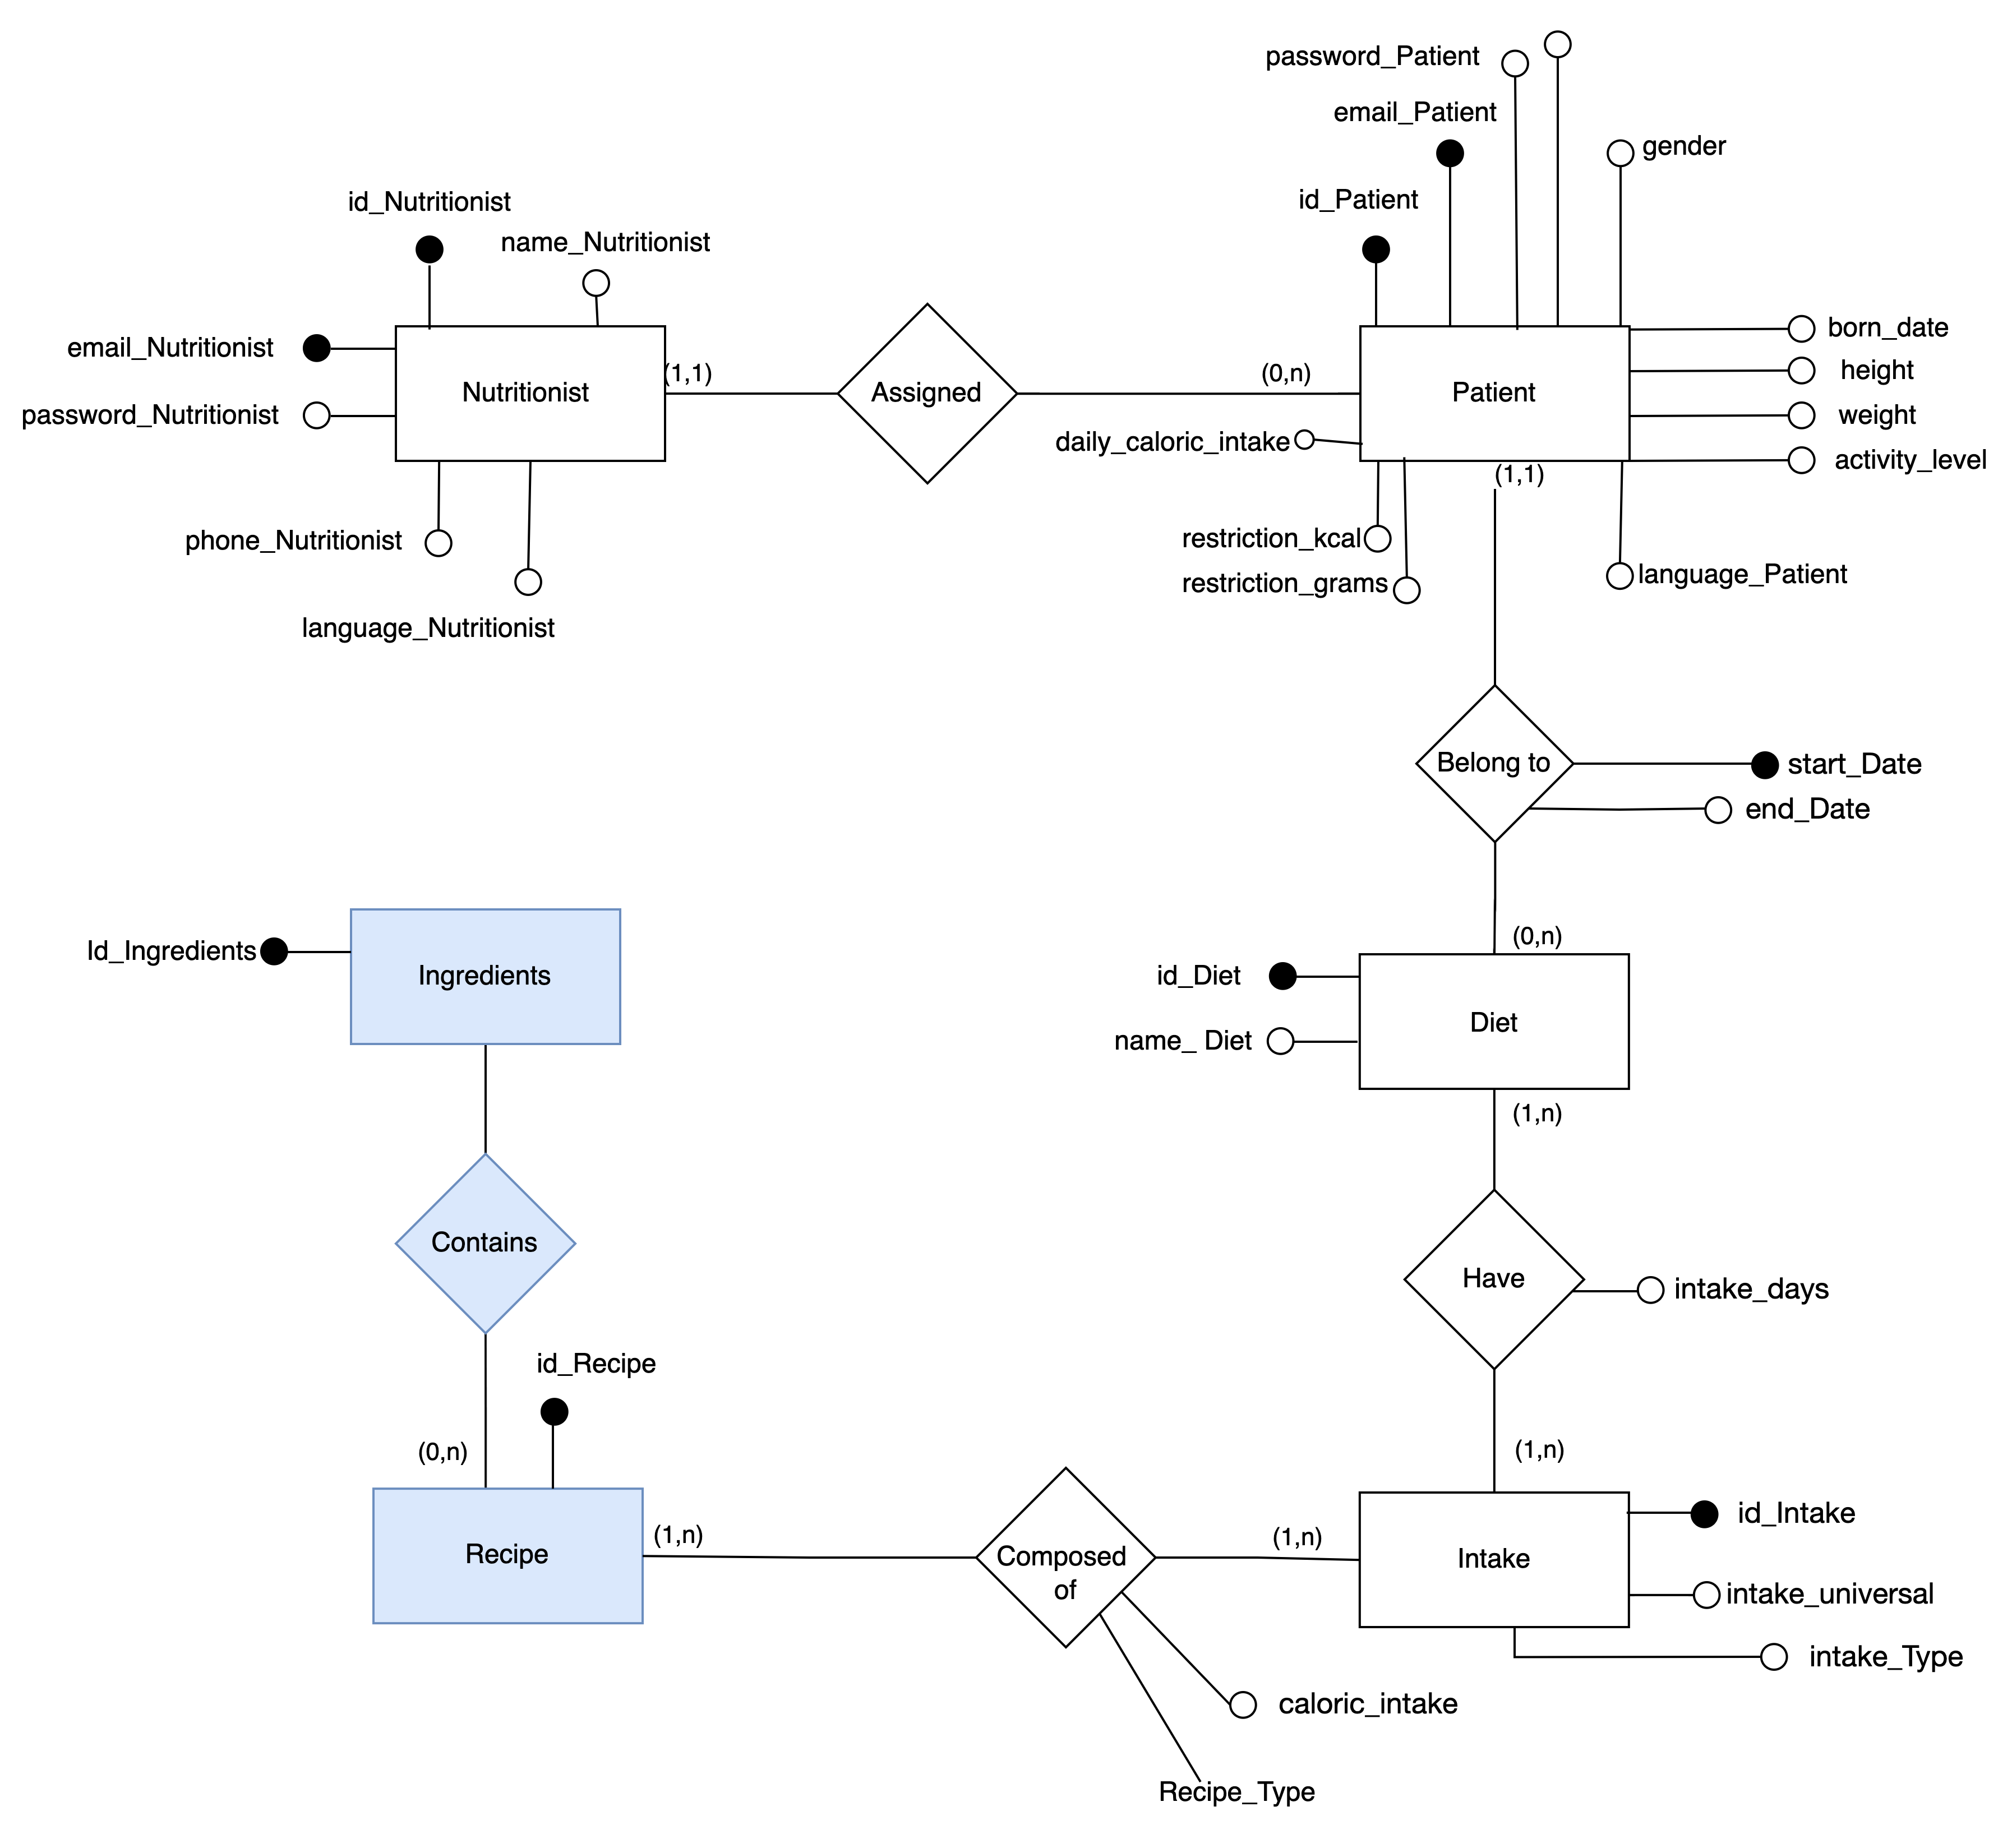
\includegraphics[width=1\linewidth]{Plantilla_TFG_latex/imagenes/DiagramaE_R.png}
    \caption{Diagrama conceptual}
    \label{fig:enter-label}
\end{figure}

\section{Casos de uso}
En esta sección se describen los principales casos de uso del sistema de información. Estos casos de uso reflejan las interacciones típicas que los usuarios (nutricionistas) pueden realizar con el sistema a través de la interfaz web desarrollada con React, en comunicación con una API basada en FastAPI y una base de datos MongoDB.

\subsection{Resumen de casos de uso por módulo}
A continuación, se presenta una visión general de los principales casos de uso organizados por módulo funcional del sistema:

\subsubsection*{Módulo: Autenticación (``auth'')}

\begin{table}[H]
\centering
\begin{tabular}{|c|p{7.5cm}|c|}
\hline
\textbf{ID} & \textbf{Nombre del caso de uso} & \textbf{Actor principal} \\
\hline
CU-A01 & Registro de nutricionista & Nutricionista \\
\hline
CU-A02 & Inicio de sesión (``login'') & Nutricionista \\
\hline
CU-A03 & Renovación de token de acceso (``refresh token'') & Nutricionista \\
\hline
CU-A04 & Obtener perfil del usuario actual & Nutricionista \\
\hline
\end{tabular}
\caption{Casos de uso del módulo de autenticación}
\end{table}

\subsubsection*{Módulo: Gestión de ingredientes (``ingredient'')}

\begin{table}[H]
\centering
\begin{tabular}{|c|p{7.5cm}|c|}
\hline
\textbf{ID} & \textbf{Nombre del caso de uso} & \textbf{Actor principal} \\
\hline
CU-I01 & Obtener todas las categorías de alimentos & Nutricionista \\
\hline
CU-I02 & Buscar alimentos por nombre o palabra clave & Nutricionista \\
\hline
CU-I03 & Obtener alimentos por categoría & Nutricionista \\
\hline
CU-I04 & Obtener detalles de un alimento específico & Nutricionista \\
\hline
CU-I05 & Sugerir alimentos similares (semánticamente) & Nutricionista \\
\hline
CU-I06 & Obtener porciones estándar de un alimento & Nutricionista \\
\hline
CU-I07 & Actualizar o consultar imagen asociada al alimento & Nutricionista \\
\hline
\end{tabular}
\caption{Casos de uso del módulo de ingredientes}
\end{table}

\subsubsection*{Módulo: Gestión de Recetas (``recipes'')}

\begin{table}[H]
\centering
\begin{tabular}{|c|p{7.5cm}|c|}
\hline
\textbf{ID} & \textbf{Nombre del caso de uso} & \textbf{Actor principal} \\
\hline
CU-R01 & Buscar recetas por nombre o palabra clave & Nutricionista \\
\hline
CU-R02 & Listar recetas por categoría & Nutricionista \\
\hline
CU-R03 & Ver detalle completo de una receta & Nutricionista \\
\hline
CU-R04 & Obtener valores nutricionales por ración o totales & Nutricionista \\
\hline
CU-R05 & Sugerir recetas similares por embeddings & Nutricionista \\
\hline
CU-R06 & Obtener recetas con resumen nutricional filtrado & Nutricionista \\
\hline
CU-R07 & Calcular máximos nutricionales por categoría & Nutricionista \\
\hline
\end{tabular}
\caption{Casos de uso del módulo \texttt{recipe}}
\end{table}

\subsubsection*{Módulo: Gestión de Ingestas (``intakes'')}

\begin{table}[H]
\centering
\begin{tabular}{|c|p{7.5cm}|c|}
\hline
\textbf{ID} & \textbf{Nombre del caso de uso} & \textbf{Actor principal} \\
\hline
CU-IN01 & Crear ingesta personalizada para un paciente & Nutricionista \\
\hline
CU-IN02 & Editar una ingesta existente & Nutricionista \\
\hline
CU-IN03 & Ver ingestas de un paciente (y universales) & Nutricionista \\
\hline
CU-IN04 & Ver detalle de una ingesta por ID o nombre & Nutricionista \\
\hline
CU-IN05 & Buscar ingestas por nombre & Nutricionista \\
\hline
CU-IN06 & Eliminar ingesta existente & Nutricionista \\
\hline
\end{tabular}
\caption{Casos de uso del módulo \texttt{intake}}
\end{table}

\subsubsection*{Módulo: Gestión de dietas (``diet'')}

\begin{table}[H]
\centering
\begin{tabular}{|c|p{7.5cm}|c|}
\hline
\textbf{ID} & \textbf{Nombre del caso de uso} & \textbf{Actor principal} \\
\hline
CU-D01 & Crear dieta para un paciente & Nutricionista \\
\hline
CU-D02 & Consultar todas las dietas de un paciente & Nutricionista \\
\hline
CU-D03 & Consultar detalle completo de una dieta & Nutricionista \\
\hline
CU-D04 & Editar una dieta existente & Nutricionista \\
\hline
CU-D05 & Eliminar una dieta existente & Nutricionista \\
\hline
\end{tabular}
\caption{Casos de uso del módulo de gestión de dietas}
\end{table}

\subsubsection*{Módulo: Gestión de Pacientes (``pacient'')}

\begin{table}[H]
\centering
\begin{tabular}{|c|p{7.5cm}|c|}
\hline
\textbf{ID} & \textbf{Nombre del caso de uso} & \textbf{Actor principal} \\
\hline
CU-P01 & Crear paciente con cálculo nutricional inicial & Nutricionista \\
\hline
CU-P02 & Listar pacientes asignados al nutricionista & Nutricionista \\
\hline
CU-P03 & Consultar información nutricional de un paciente & Nutricionista \\
\hline
CU-P04 & Actualizar datos y valores nutricionales del paciente & Nutricionista \\
\hline
CU-P05 & Eliminar paciente del sistema & Nutricionista \\
\hline
\end{tabular}
\caption{Casos de uso del módulo \texttt{pacient}}
\end{table}



